\frame
{
	\begin{center}
		\Large Kommunikationskostenoptimierung \normalsize
	\end{center}
}
\frame
{
	\frametitle{Motivation}
	\begin{figure}[h!]
		\centering
		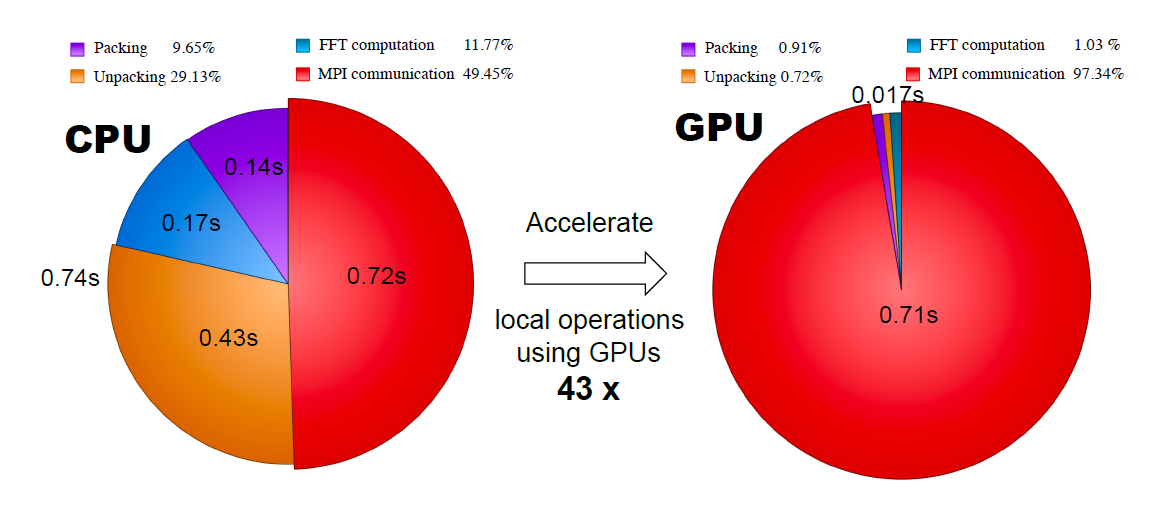
\includegraphics[width=\linewidth, keepaspectratio]{../res/speedup.png}
	\end{figure}

	\begin{itemize}
		\item $\frac{0.14s+0.17s+0.42s+0.72s}{0.017s+0.71s}=200,8\% \rightarrow$  2-fache Beschleunigung
		\item Kommunikationszeit nur vernachlässigbare Änderung
		\item rechte Seite graphisch nicht akkurat dargestellt!
	\end{itemize}
}
\frame
{
	\frametitle{Bottleneck: Kommunikation}
	Nach der Beschleunigung ist der  Zeitanteil der Kommunikation:\\
	$$\frac{0.71s}{0.71s+0.017}\approx97,6\%$$
	$\implies$ Bottleneck in der Kommunikation\\
	\large Was tun? \normalsize
}
\frame
{
	\frametitle{Was tun?}
	Konzeptionell 2 Ansätze:
	\begin{itemize}
		\item Option1: Verwendung eines besseren Algorithmus hinsichtlich serieller Anteile und Kommunikation.
		\item Option2: Verbesserung der Kommunikationsstrategie unter Einbeziehung von Eigenschaften der Systemarchitektur.
	\end{itemize}
}
\frame
{
	\frametitle{Ansatz 1}
	Nach Option2: Untersuchung Kommunikativer Eigenschaften der Systemarchitektur
	\begin{figure}[h!]
		\centering
		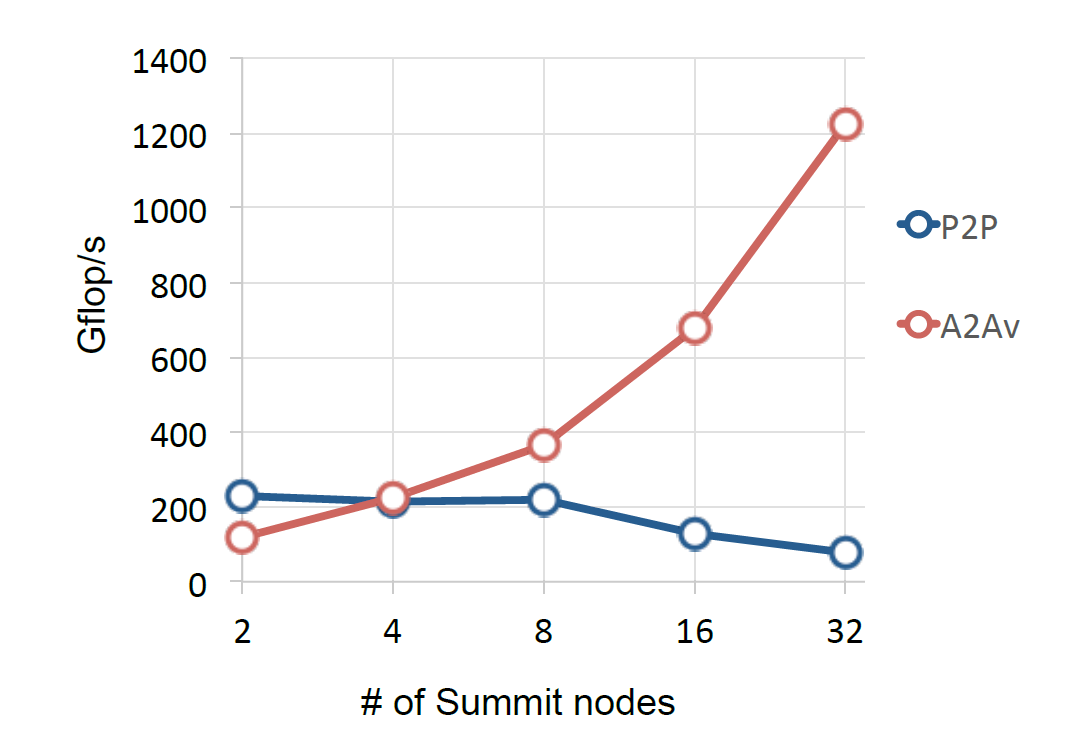
\includegraphics[width=0.7\linewidth, keepaspectratio]{./res/bench.png}
	\end{figure}
}
\frame
{
	\frametitle{Ansatz 2}
	Nach Option1: Algorithmische Anpassung
	\begin{figure}[h!]
		\centering
		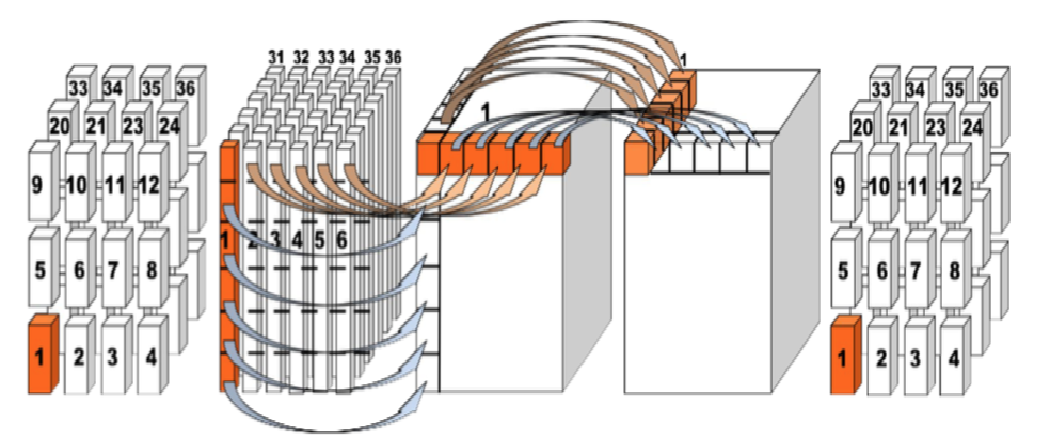
\includegraphics[width=0.7\linewidth, keepaspectratio]{../res/algo.png}
	\end{figure}
	1D\textit{pencil} $\rightarrow$ 2D\textit{slabs} Übertragungsgröße
	$(TransformX,TransformY,TransformZ,MoveBack)\rightarrow(TransformY,TransformZ,MoveBack)$
	Theretisch: $25\%$ Ersparnis
}

\frame
{
	\frametitle{Ansatz 2}
	\begin{figure}[h!]
		\centering
		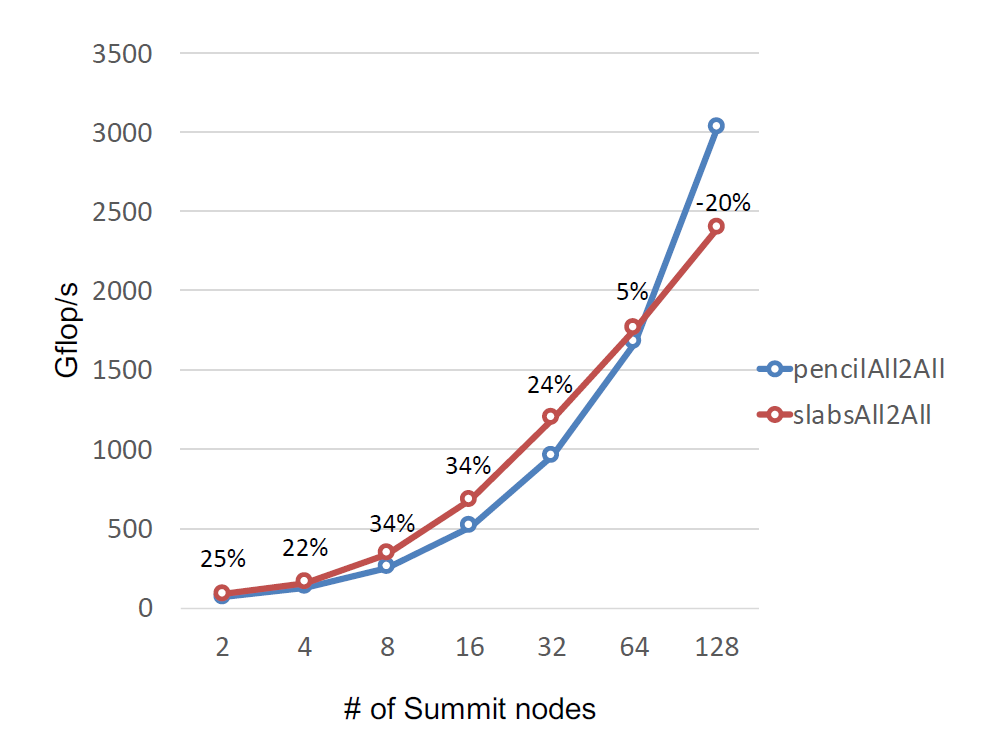
\includegraphics[width=0.7\linewidth, keepaspectratio]{./res/bench2.png}
	\end{figure}
	Nachteil: Quadratischer Speicherverbrauch pro Knoten
}
